%\documentstyle[epsf,twocolumn]{jarticle}       %LaTeX2e仕様
\documentclass[twocolumn]{jarticle}     %pLaTeX2e仕様(platex.exeの場合)
%\documentclass[twocolumn]{ujarticle}     %pLaTeX2e仕様(uplatex.exeの場合)
%%%%%%%%%%%%%%%%%%%%%%%%%%%%%%%%%%%%%%%%%%%%%%%%%%%%%%%%%%%%%%
%%
%%  基本バージョン
%%
%%%%%%%%%%%%%%%%%%%%%%%%%%%%%%%%%%%%%%%%%%%%%%%%%%%%%%%%%%%%%%%%
\setlength{\topmargin}{-45pt}
%\setlength{\oddsidemargin}{0cm} 
\setlength{\oddsidemargin}{-7.5mm}
%\setlength{\evensidemargin}{0cm} 
\setlength{\textheight}{24.1cm}
%setlength{\textheight}{25cm} 
\setlength{\textwidth}{17.4cm}
%\setlength{\textwidth}{172mm} 
\setlength{\columnsep}{11mm}

\kanjiskip=.07zw plus.5pt minus.5pt


% 【節が変わるごとに (1.1)(1.2) … (2.1)(2.2) と数式番号をつけるとき】
%\makeatletter
%\renewcommand{\theequation}{%
%\thesection.\arabic{equation}} %\@addtoreset{equation}{section}
%\makeatother

%\renewcommand{\arraystretch}{0.95} 行間の設定

%%%%%%%%%%%%%%%%%%%%%%%%%%%%%%%%%%%%%%%%%%%%%%%%%%%%%%%%
\usepackage[dvipdfmx]{graphicx}   %pLaTeX2e仕様(\documentstyle ->\documentclass)\documentclass[dvipdfmx]{graphicx}
\usepackage[dvipdfmx]{color}
\usepackage[subrefformat=parens]{subcaption}
\usepackage{colortbl}
\usepackage{multicol}
%%%%%%%%%%%%%%%%%%%%%%%%%%%%%%%%%%%%%%%%%%%%%%%%%%%%%%%%

\begin{document}

\twocolumn[
\noindent

\hspace{1em}
2020年12月18日
\hfill
\ \ 細川 岳大

\vspace{2mm}

\hrule

\begin{center}
{\Large \bf 進捗報告}
\end{center}
\hrule
\vspace{3mm}
]

% ‚ここから 文章 Start!

\section{今週やったこと}

\begin{itemize}
	\item GAの実験
	\item 論文の再調査
\end{itemize}

\section{GAの実験}
表\ref{tb:GApara},\ref{tb:FTXpara}に実験の設定を示す.
遺伝子は0から9の整数値をとる整数値コーディングとした.\\
選択はサイズ2のトーナメント選択,交叉には二点交叉,突然変異は別の数値にランダムに移るように設定した.\\
また,今回事前学習したモデルを初期モデルとして学習させた.
前回言われていたように, softmax 値から初期個体を生成した.

\begin{table}[h]
	\centering
	\caption{GAの設定\label{tb:GApara}}
	\scalebox{1.0}{
		\begin{tabular}{|c||c|} \hline
			個体数&20\\ \hline
			世代数&13\\ \hline
			交叉率&1.0\\ \hline
			突然変異率&0.02\\ \hline\hline
			labeled&250枚\\ \hline
			search&100枚\\ \hline
		\end{tabular}
	}
\end{table}

\begin{table}[h]
	\centering
	\caption{FixMatchの設定\label{tb:FTXpara}}
	\scalebox{1.0}{
		\begin{tabular}{|c|c|c|} \hline
			model&\multicolumn{2}{c|}{WideResNet16-2}\\ \hline\hline
			data set&\multicolumn{2}{c|}{cifar10}\\ \hline
			batch size&labeled&32\\ \cline{2-3}
			&unlabeled&$32*7$\\ \hline
			optimizer&\multicolumn{2}{c|}{SGD(lr=0.1,momntum=0.9)}\\ \hline
			loss&\multicolumn{2}{c|}{cross\_entropy\_loss}\\ \hline\hline
			\multicolumn{3}{|c|}{事前学習}\\ \hline
			train &labeled&100\\ \cline{2-3}
			&unlabeled&49650\\ \hline			
			val data&\multicolumn{2}{c|}{150}\\ \hline
			num\_iterations&\multicolumn{2}{c|}{2**16}\\ \hline\hline
			\multicolumn{3}{|c|}{GAの評価}\\ \hline
			train &searchのみ&100\\ \cline{2-3}
			&unlabeled&49650\\ \hline
			val data&\multicolumn{2}{c|}{250}\\ \hline
			num\_iterations&\multicolumn{2}{c|}{5000}\\ \hline
		\end{tabular}
	}
\end{table}


\subsection{結果}
図\ref{fig:ex1},\ref{fig:ex1_1}に示す.
正答数が下がっているのは分かるが,適応度に関してもかなりばらつきがあり,
初期個体に比べ下がってしまっていることがわかる.


\begin{figure}[h]
	\begin{center}
		\vspace*{-3mm}
		\hspace*{-12mm}
		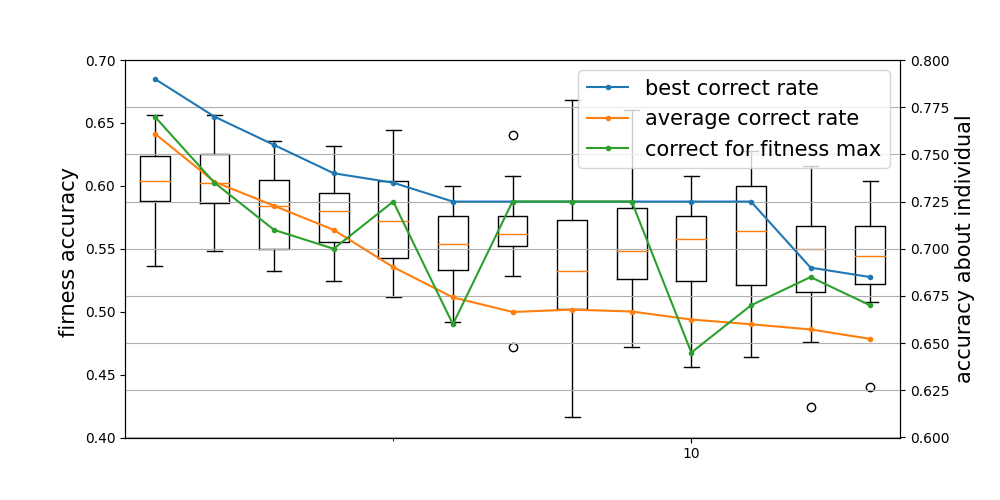
\includegraphics[height=65mm,width=100mm]{graph.png}
		\caption{実験1の結果\label{fig:ex1}}
	\end{center}
\end{figure}
\begin{figure}[h]
	\begin{center}
		\vspace*{-3mm}
		\hspace*{-12mm}
		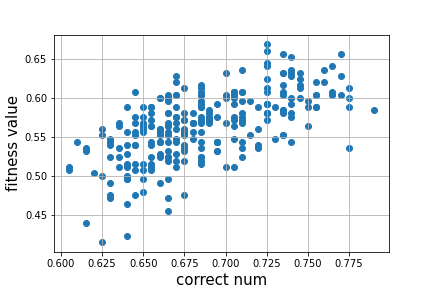
\includegraphics[height=65mm,width=100mm]{img.png}
		\caption{実験1の相関図\label{fig:ex1_1}}
	\end{center}
\end{figure}




\section{論文の再調査}
先々週にも軽く紹介したが,半教師あり学習(Semi Supervised Learning:semi-SL) に対し,
自己教師あり学習(Self Supervised Learning:self-SL)という自動で生成できる情報によって特徴マップを学習する手法を取り入れたものが性能を示している.

\subsection{対象学習(Contrastive Learning:CL)}
CLは同じ画像の異なる変換画像から得られる特徴マップを一致するように,また,異なる画像の特徴マップから離れさせるように学習する手法である.

\subsection{A Simple Framework for Contrastive Learning of Visual Representations(:SimCLR)}
SimCLR は encoder,projection head を CL を用いて学習し,得られたエンコーダに MLP などの分類器をつけてラベル付きデータでファインチューニングをするものである.また,精度を出すためにはエンコーダもバッチサイズも非常に大きなものが必要となる.

\begin{figure}[h]
	\begin{center}
		\vspace*{-3mm}
		\hspace*{-12mm}
		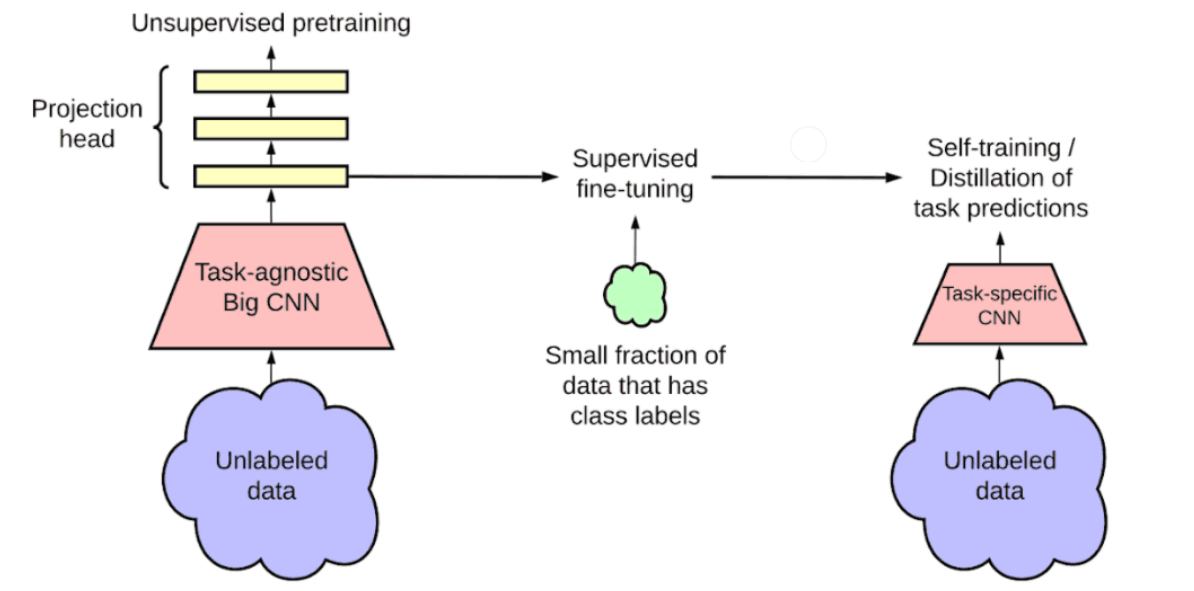
\includegraphics[height=65mm,width=100mm]{キャプチャ.PNG}
		\caption{SimCLRの概略図\label{fig:}}
	\end{center}
\end{figure}

\subsection{Ensemble AutoEncoding Transformers(:EnAET)}
EnAET はエンコーダ部が一つでデコーダ部が複数の AutoEncoder を用いて学習を行う.
\begin{figure}[h]
	\begin{center}
		\vspace*{-3mm}
		\hspace*{-12mm}
		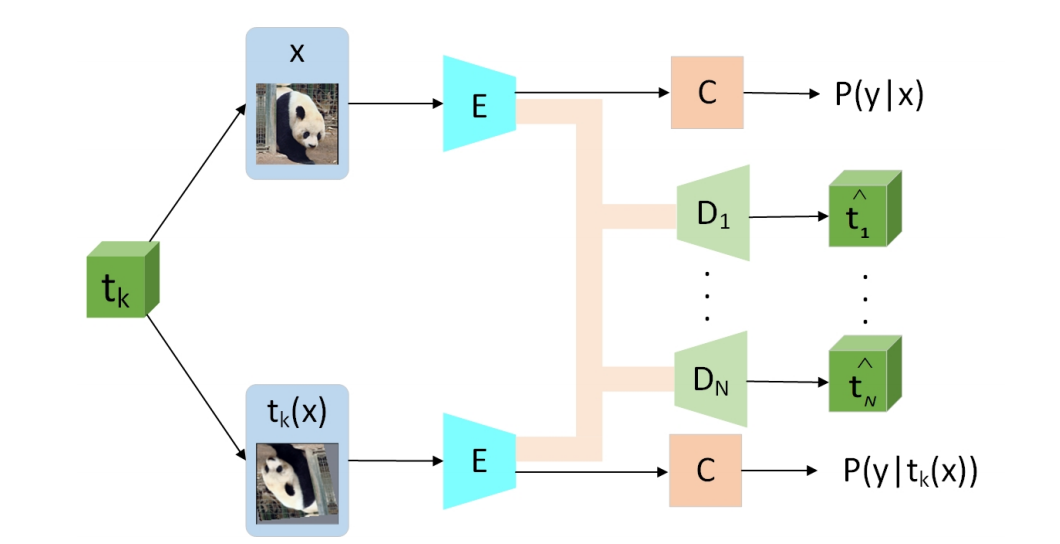
\includegraphics[height=65mm,width=100mm]{EnAET.png}
		\caption{EnAETの概略図\label{fi:}}
	\end{center}
\end{figure}

\subsection{CoMatch}
CoMatch は SimCLR における projection head と分類器を同時に学習させていく手法で,
その際に FixMatch の疑似ラベルを用いて学習する.
また,非常に大きいバッチサイズを解決するために, Momentum Contrastive Learning を用いる.

\begin{figure}[h]
	\begin{center}
		\vspace*{-3mm}
		\hspace*{-12mm}
		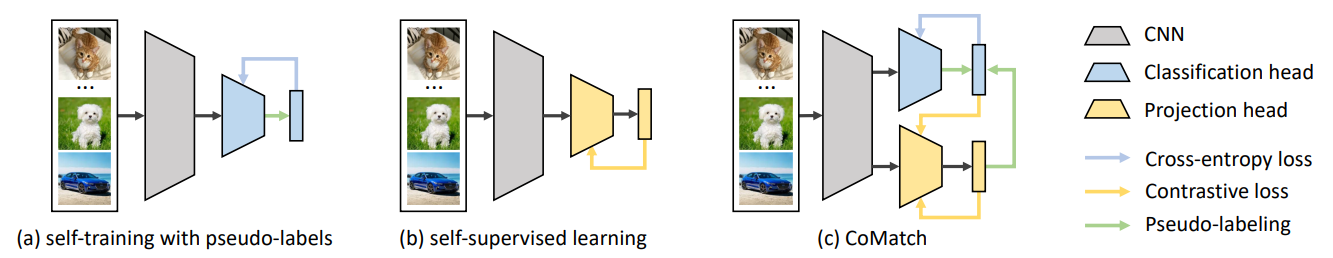
\includegraphics[height=50mm,width=200mm]{CoMatch.png}
		\caption{CoMatchの概略図\label{i:}}
	\end{center}
\end{figure}

\section{来週の課題}
\begin{itemize}
	\item 実験設定の改良
\end{itemize}

\end{document}


